\chapter{PK3 --- Hồ sơ \& mục tiêu}
\clearpage\begin{landscape}
\begin{figure}[H]\centering
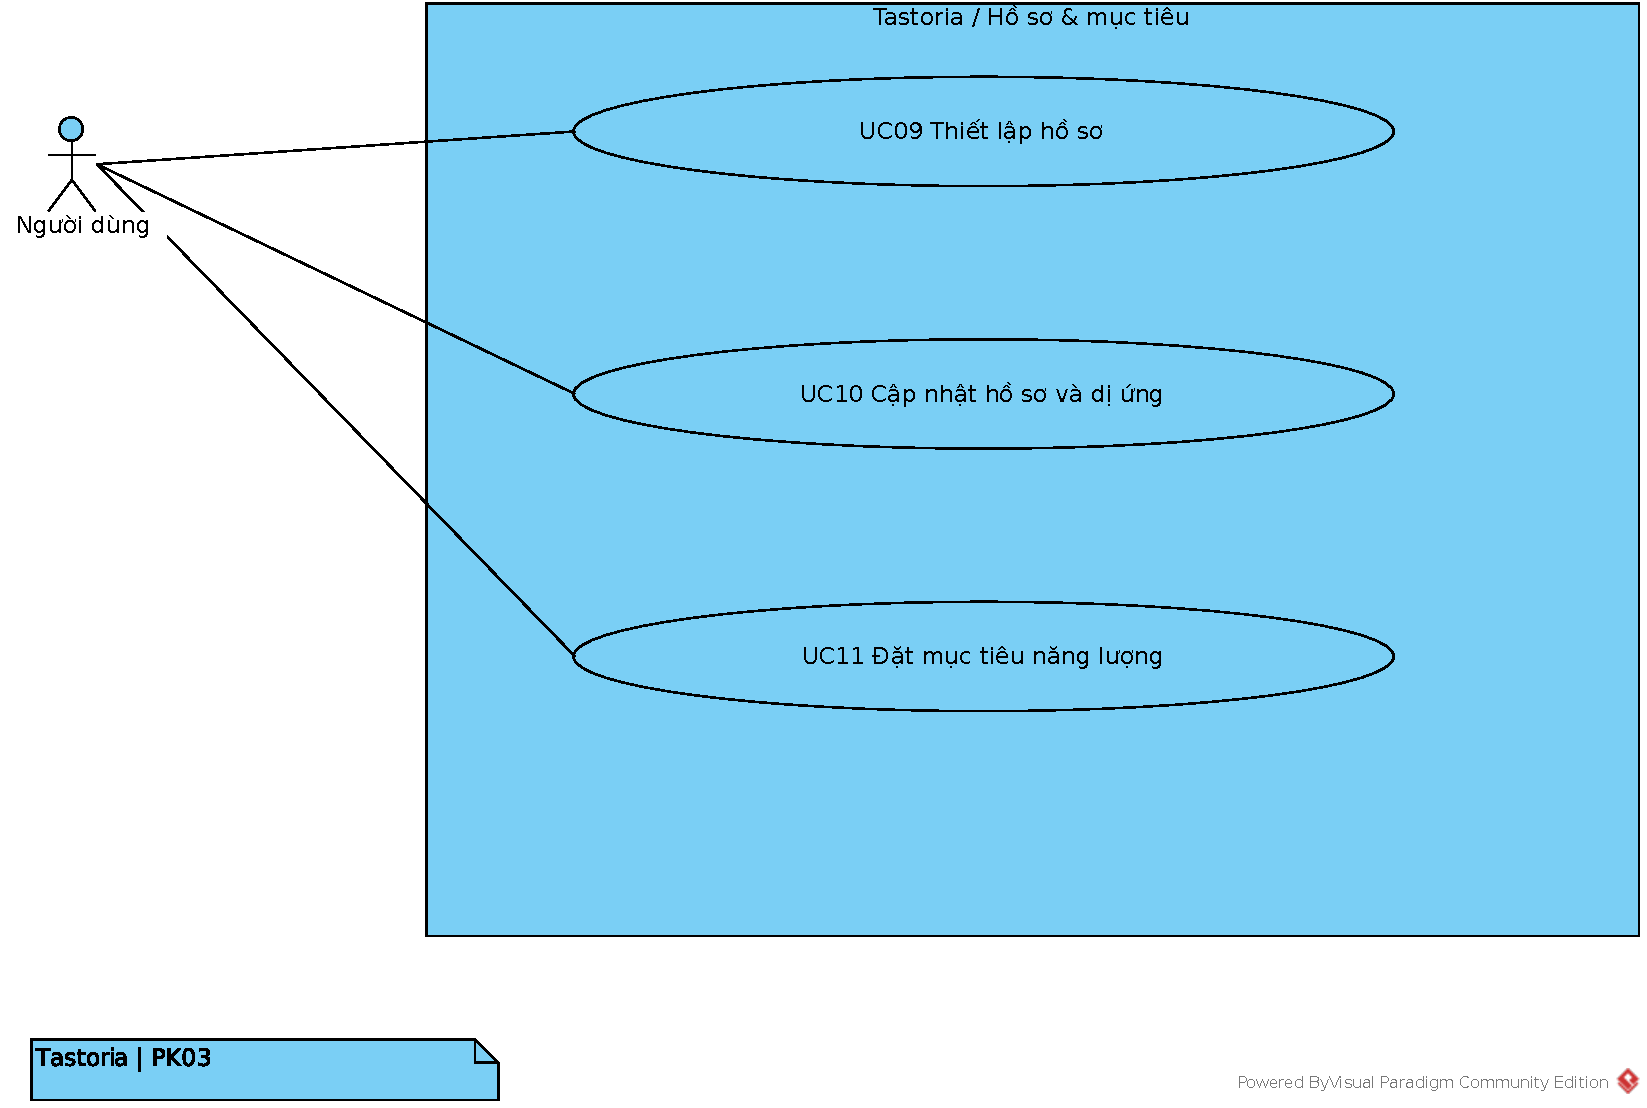
\includegraphics[width=0.96\linewidth,height=0.78\textwidth,keepaspectratio]{assets/PK03.pdf}
\caption{PK03 --- Phân rã use case}\label{fig:Phu-luc-A-Use-Cases:3}
\end{figure}
\end{landscape}\clearpage
\section{UC09 --- Thiết lập hồ sơ 60 giây}
\subsection{Mục tiêu trong ngữ cảnh}
Người dùng (A02) vừa có tài khoản cần, trong khoảng một phút, khai đủ thông tin để Tastoria ghép được mâm cơm an toàn và vừa năng lượng: đồng ý theo mục đích, chỉ số cơ thể, mức vận động, mục tiêu năng lượng, dị ứng, chế độ ăn và 5 món hay ăn. Màn này chỉ xuất hiện lần đầu; sửa về sau thuộc UC10 và UC11.

\subsection{Phạm vi và mức}
\begin{itemize}
\item Phạm vi: hệ thống Tastoria (app Android/\allowbreak{}web + backend), hộp đen.
\item Mức: mục tiêu người dùng (sea level).
\item Gói: PK3 Hồ sơ \& mục tiêu.
\end{itemize}
\subsection{Tác nhân và bên liên quan (quyền lợi)}
{\footnotesize\setlength{\tabcolsep}{0pt}
\begin{longtable}{@{}L{7.850cm}@{\hspace{3mm}}L{7.850cm}@{}}
\caption{Tác nhân và bên liên quan (quyền lợi)}\\
\toprule
\textbf{Tác nhân /\allowbreak{} bên liên quan} & \textbf{Quyền lợi} \\
\midrule\endfirsthead
\multicolumn{2}{l}{\small\itshape Bảng \thetable{} (tiếp theo)}\\
\toprule
\textbf{Tác nhân /\allowbreak{} bên liên quan} & \textbf{Quyền lợi} \\
\midrule\endhead
\bottomrule\endfoot
A02 Người dùng (chính) & Khai nhanh, ít trường; biết rõ dữ liệu nào bị dùng cho mục đích nào; có thể bỏ qua phần sức khỏe mà vẫn dùng được app. \\ \addlinespace[3pt]
Người ăn cùng (không tài khoản) & Không bị đề xuất món thuộc nhóm dị ứng người dùng đã khai cho chính mình (dị ứng người ăn cùng khai theo bữa ở UC15). \\ \addlinespace[3pt]
Nhóm phát triển (chủ thể chịu trách nhiệm xử lý dữ liệu) & Có bằng chứng đồng ý gắn phiên bản điều khoản; chỉ số cơ thể chỉ lưu khi có đồng ý {\small\texttt{health\_\allowbreak{}\allowbreak{}profile}} và luôn ở dạng mã hoá. \\ \addlinespace[3pt]
Nhóm Học máy & Có 5 món hay ăn làm đặc trưng người dùng cho xếp hạng gu lúc khởi đầu lạnh. \\ \addlinespace[3pt]
\end{longtable}}
\subsection{Tiền điều kiện}
\begin{itemize}
\item A02 đã đăng nhập (UC01 hoặc UC02) và có access token còn hạn.
\item Tài khoản chưa có dòng {\small\texttt{profiles}} (app kiểm bằng {\small\texttt{GET /\allowbreak{}\allowbreak{}me/\allowbreak{}\allowbreak{}profile}} của UC10 trả hồ sơ rỗng).
\item Bảng {\small\texttt{consent\_\allowbreak{}\allowbreak{}purposes}} có 4 mục đích và mỗi mục đích có một {\small\texttt{policy\_\allowbreak{}\allowbreak{}versions}} đang hiệu lực; bảng {\small\texttt{allergen\_\allowbreak{}\allowbreak{}groups}}, {\small\texttt{diets}} và ít nhất một món {\small\texttt{recipes.\allowbreak{}status = published}} đã được nạp (UC25).
\end{itemize}
\subsection{Đảm bảo tối thiểu}
\begin{itemize}
\item Không lưu chỉ số cơ thể nào khi chưa có đồng ý {\small\texttt{health\_\allowbreak{}\allowbreak{}profile}} hiện hành.
\item Chỉ số cơ thể không bao giờ được lưu ở dạng rõ; mỗi lần giải mã có một dòng {\small\texttt{audit\_\allowbreak{}\allowbreak{}log}}.
\item Bước nào đã được hệ thống xác nhận lưu (HTTP 200) thì giữ nguyên khi app bị tắt giữa chừng; bước lỗi không để lại dữ liệu dở dang.
\end{itemize}
\subsection{Đảm bảo khi thành công}
\begin{itemize}
\item {\small\texttt{consent\_\allowbreak{}\allowbreak{}events}} có một sự kiện {\small\texttt{grant}} (kênh {\small\texttt{onboarding}}) cho mỗi mục đích người dùng chọn, gắn đúng {\small\texttt{policy\_\allowbreak{}\allowbreak{}version\_\allowbreak{}\allowbreak{}id}} hiện hành.
\item Nếu có đồng ý {\small\texttt{health\_\allowbreak{}\allowbreak{}profile}}: {\small\texttt{profiles}} có các cột {\small\texttt{*\_\allowbreak{}\allowbreak{}enc}}, {\small\texttt{enc\_\allowbreak{}\allowbreak{}key\_\allowbreak{}\allowbreak{}id}}, {\small\texttt{activity\_\allowbreak{}\allowbreak{}level}}, {\small\texttt{goal}}, {\small\texttt{kcal\_\allowbreak{}\allowbreak{}target}}, {\small\texttt{kcal\_\allowbreak{}\allowbreak{}source}}.
\item {\small\texttt{user\_\allowbreak{}\allowbreak{}allergens}} chứa đúng tập nhóm dị ứng đã chọn (có thể rỗng khi người dùng chọn "Không dị ứng nhóm nào"); {\small\texttt{profiles.\allowbreak{}diet\_\allowbreak{}\allowbreak{}code}} đúng lựa chọn.
\item {\small\texttt{user\_\allowbreak{}\allowbreak{}favorite\_\allowbreak{}\allowbreak{}recipes}} có 0--5 món đã xuất bản.
\item App chuyển tới Trang chủ.
\end{itemize}
\subsection{Kích hoạt}
\begin{itemize}
\item Ngay sau khi UC01 Đăng ký tài khoản thành công; hoặc
\item A02 đăng nhập (UC02) trên thiết bị mới khi tài khoản chưa có hồ sơ.
\end{itemize}
\subsection{Kịch bản chính}
\begin{enumerate}
\item \textbf{App} lấy văn bản điều khoản hiện hành của từng mục đích {\small\texttt{health\_\allowbreak{}\allowbreak{}profile}}, {\small\texttt{personalization}}, {\small\texttt{photo\_\allowbreak{}\allowbreak{}contribution}} qua {\small\texttt{GET /\allowbreak{}\allowbreak{}policies/\allowbreak{}\allowbreak{}\{purpose\}/\allowbreak{}\allowbreak{}current}} (module privacy) và hiện màn đồng ý riêng, mỗi mục đích một ô chưa tích. \textbf{[đồng ý theo từng mục đích; người dùng có thể bỏ qua phần không bắt buộc]}
\item \textbf{A02} tích các mục đích muốn đồng ý và bấm "Tiếp tục".
\item \textbf{App} gửi {\small\texttt{POST /\allowbreak{}\allowbreak{}me/\allowbreak{}\allowbreak{}consents}} với danh sách (mục đích, {\small\texttt{policy\_\allowbreak{}\allowbreak{}version\_\allowbreak{}\allowbreak{}id}}, {\small\texttt{grant}}), kênh {\small\texttt{onboarding}}. \textbf{Module privacy} ghi {\small\texttt{consent\_\allowbreak{}\allowbreak{}events}} và trả trạng thái hiện hành từ {\small\texttt{v\_\allowbreak{}\allowbreak{}current\_\allowbreak{}\allowbreak{}consents}}.
\item \textbf{App} hiện thanh tiến độ 4 bước và bước 1 "Cơ thể": giới, năm sinh, chiều cao, cân nặng. \textbf{A02} nhập và bấm "Tiếp".
\item \textbf{App} hiện bước 2 "Vận động và mục tiêu": mức vận động (nhẹ /\allowbreak{} trung bình /\allowbreak{} nặng) và mục tiêu (giữ cân /\allowbreak{} giảm cân /\allowbreak{} do chuyên gia đặt). \textbf{A02} chọn và bấm "Tiếp".
\item \textbf{App} gửi {\small\texttt{PUT /\allowbreak{}\allowbreak{}me/\allowbreak{}\allowbreak{}profile}}. \textbf{Module profile} gọi {\small\texttt{privacy.\allowbreak{}has\_\allowbreak{}\allowbreak{}consent(user\_\allowbreak{}\allowbreak{}id, "health\_\allowbreak{}\allowbreak{}profile")}}, kiểm tuổi \ensuremath{\geq} 18 và miền giá trị, mã hoá AES-\allowbreak{}GCM các cột {\small\texttt{sex\_\allowbreak{}\allowbreak{}enc}}, {\small\texttt{birth\_\allowbreak{}\allowbreak{}year\_\allowbreak{}\allowbreak{}enc}}, {\small\texttt{height\_\allowbreak{}\allowbreak{}cm\_\allowbreak{}\allowbreak{}enc}}, {\small\texttt{weight\_\allowbreak{}\allowbreak{}kg\_\allowbreak{}\allowbreak{}enc}}, ghi {\small\texttt{enc\_\allowbreak{}\allowbreak{}key\_\allowbreak{}\allowbreak{}id}}, {\small\texttt{activity\_\allowbreak{}\allowbreak{}level}}, {\small\texttt{goal}} vào {\small\texttt{profiles}}.
\item \textbf{App} gửi {\small\texttt{POST /\allowbreak{}\allowbreak{}me/\allowbreak{}\allowbreak{}energy-\allowbreak{}suggestion}}. \textbf{Module profile} giải mã chỉ số (gọi {\small\texttt{privacy.\allowbreak{}audit(.\allowbreak{}.\allowbreak{}.\allowbreak{})}} để ghi {\small\texttt{audit\_\allowbreak{}\allowbreak{}log}}), tính BMR, TEE, E theo FR-\allowbreak{}11-\allowbreak{}01 đến FR-\allowbreak{}11-\allowbreak{}05 và E\_\allowbreak{}mâm trưa/\allowbreak{}tối theo FR-\allowbreak{}11-\allowbreak{}08, trả kết quả mà không ghi {\small\texttt{profiles}}.
\item \textbf{App} hiện mục tiêu gợi ý (kcal/\allowbreak{}ngày, E\_\allowbreak{}mâm trưa và tối, dòng "đây là ước tính" kèm nguồn công thức). \textbf{A02} bấm "Dùng mục tiêu này".
\item \textbf{App} gửi {\small\texttt{PUT /\allowbreak{}\allowbreak{}me/\allowbreak{}\allowbreak{}energy-\allowbreak{}target}} với {\small\texttt{kcal\_\allowbreak{}\allowbreak{}source = suggested}}. \textbf{Module profile} tính lại E từ hồ sơ đã lưu và ghi {\small\texttt{kcal\_\allowbreak{}\allowbreak{}target}}, {\small\texttt{kcal\_\allowbreak{}\allowbreak{}source}}.
\item \textbf{App} lấy {\small\texttt{GET /\allowbreak{}\allowbreak{}reference}} (module catalog: {\small\texttt{allergen\_\allowbreak{}\allowbreak{}groups}}, {\small\texttt{diets}}) và hiện bước 3 "Dị ứng và chế độ ăn". \textbf{A02} chọn các nhóm dị ứng (hoặc "Không dị ứng nhóm nào") và chế độ ăn (không có /\allowbreak{} chay), bấm "Tiếp".
\item \textbf{App} gửi {\small\texttt{PUT /\allowbreak{}\allowbreak{}me/\allowbreak{}\allowbreak{}allergens}} rồi {\small\texttt{PUT /\allowbreak{}\allowbreak{}me/\allowbreak{}\allowbreak{}diet}}. \textbf{Module profile} gọi catalog để kiểm mã và ghi {\small\texttt{user\_\allowbreak{}\allowbreak{}allergens}}, {\small\texttt{profiles.\allowbreak{}diet\_\allowbreak{}\allowbreak{}code}}.
\item \textbf{App} lấy {\small\texttt{GET /\allowbreak{}\allowbreak{}recipes}} (module catalog, chỉ món {\small\texttt{published}}) và hiện bước 4 "5 món hay ăn". \textbf{A02} chọn tối đa 5 món và bấm "Xong".
\item \textbf{App} gửi {\small\texttt{PUT /\allowbreak{}\allowbreak{}me/\allowbreak{}\allowbreak{}favorites}}. \textbf{Module profile} kiểm số lượng và trạng thái món qua catalog, ghi {\small\texttt{user\_\allowbreak{}\allowbreak{}favorite\_\allowbreak{}\allowbreak{}recipes}}.
\item \textbf{App} chuyển tới Trang chủ. Use case kết thúc.
\end{enumerate}
\subsection{Mở rộng}
\begin{itemize}
\item \textbf{1a.} Không lấy được điều khoản (mất mạng, 5xx): app hiện "Không tải được điều khoản" và nút "Thử lại"; không cho sang bước 2. Endpoint lũy đẳng nên gọi lại an toàn.
\item \textbf{3a.} A02 không tích ô nào: hợp lệ; app vẫn gửi danh sách rỗng (không có sự kiện nào được ghi) và đi tiếp. Mọi ô đều không tích sẵn (BR-\allowbreak{}CONSENT-\allowbreak{}01).
\item \textbf{3b.} A02 không đồng ý {\small\texttt{health\_\allowbreak{}\allowbreak{}profile}}: app bỏ qua bước 1, bước 2 và các bước 6--9; hiện "Chưa có mục tiêu năng lượng" (BR-\allowbreak{}CONSENT-\allowbreak{}02); nhảy tới bước 10. Thanh tiến độ còn 2 bước.
\item \textbf{3c.} Mất mạng khi gửi {\small\texttt{POST /\allowbreak{}\allowbreak{}me/\allowbreak{}\allowbreak{}consents}}: app gửi lại cùng thân; module privacy không ghi thêm sự kiện khi trạng thái hiện hành đã khớp (hành vi của UC05). Hết 3 lần thử: app giữ lựa chọn trong máy và hiện "Thử lại".
\item \textbf{3d.} Phiên bản điều khoản đổi giữa bước 1 và 3: module privacy trả 409 {\small\texttt{policy\_\allowbreak{}\allowbreak{}version\_\allowbreak{}\allowbreak{}outdated}}; app tải lại điều khoản (quay về bước 1).
\item \textbf{5a.} A02 chọn "Do chuyên gia đặt": bước 7--8 không tính gợi ý; app hiện ô nhập kcal/\allowbreak{}ngày, gửi {\small\texttt{PUT /\allowbreak{}\allowbreak{}me/\allowbreak{}\allowbreak{}energy-\allowbreak{}target}} với {\small\texttt{kcal\_\allowbreak{}\allowbreak{}source = expert}} (quy tắc FR-\allowbreak{}11-\allowbreak{}09, FR-\allowbreak{}11-\allowbreak{}11).
\item \textbf{6a.} Năm sinh B với Y - B \ensuremath{\leq} 17 (BR-\allowbreak{}NUT-\allowbreak{}01, FR-\allowbreak{}09-\allowbreak{}05): hệ thống trả 422 {\small\texttt{age\_\allowbreak{}\allowbreak{}below\_\allowbreak{}\allowbreak{}minimum}}, không lưu gì; app hiện "Tastoria chỉ tính mục tiêu năng lượng cho người từ 18 tuổi" và cho đi tiếp như 3b.
\item \textbf{6a1.} Y - B = 18: app hỏi "Bạn đã đủ 18 tuổi chưa?"; A02 xác nhận thì app gửi lại với {\small\texttt{adult\_\allowbreak{}\allowbreak{}confirmed = true}} (FR-\allowbreak{}09-\allowbreak{}13); A02 chọn "Chưa" thì đi tiếp như 6a.
\item \textbf{6b.} Chiều cao hoặc cân nặng ngoài miền cấu hình, thiếu trường bắt buộc: 422 {\small\texttt{validation\_\allowbreak{}\allowbreak{}error}} kèm danh sách trường theo RFC 9457; app đánh dấu trường lỗi, ở lại bước 1.
\item \textbf{6c.} Đồng ý {\small\texttt{health\_\allowbreak{}\allowbreak{}profile}} vừa bị rút ở thiết bị khác (UC05): 403 {\small\texttt{consent\_\allowbreak{}\allowbreak{}required}}; app quay về màn đồng ý.
\item \textbf{6d.} Mất mạng hoặc quá thời gian khi {\small\texttt{PUT /\allowbreak{}\allowbreak{}me/\allowbreak{}\allowbreak{}profile}}: PUT lũy đẳng, app gửi lại cùng thân; kết quả cuối giống gửi một lần.
\item \textbf{6e.} Lỗi hệ thống (không lấy được khoá mã hoá, DB lỗi): 503/\allowbreak{}500 {\small\texttt{problem+json}}; giao dịch huỷ, không có dòng {\small\texttt{profiles}} dở; app hiện "Thử lại".
\item \textbf{7a.} Thiếu trường để tính (ví dụ chưa có cân nặng): 422 {\small\texttt{profile\_\allowbreak{}\allowbreak{}incomplete}} kèm tên trường; app quay về bước 1.
\item \textbf{8a.} A02 bấm "Tự nhập": app cho nhập số kcal, gửi {\small\texttt{PUT /\allowbreak{}\allowbreak{}me/\allowbreak{}\allowbreak{}energy-\allowbreak{}target}} với {\small\texttt{kcal\_\allowbreak{}\allowbreak{}source = user}} (FR-\allowbreak{}11-\allowbreak{}09, FR-\allowbreak{}11-\allowbreak{}12).
\item \textbf{8b.} A02 bấm "Để sau": không gửi bước 9; {\small\texttt{kcal\_\allowbreak{}\allowbreak{}target}} để NULL; app hiện "Chưa có mục tiêu năng lượng".
\item \textbf{10a.} A02 bấm "Tiếp" khi chưa chọn nhóm dị ứng nào và cũng chưa chọn "Không dị ứng nhóm nào": app không cho qua bước (FR-\allowbreak{}09-\allowbreak{}09).
\item \textbf{11a.} Mã dị ứng hoặc chế độ ăn không có trong {\small\texttt{allergen\_\allowbreak{}\allowbreak{}groups}}/\allowbreak{}{\small\texttt{diets}}: 422 {\small\texttt{unknown\_\allowbreak{}\allowbreak{}code}}; không ghi phần nào.
\item \textbf{12a.} A02 chọn quá 5 món: app khoá ô thứ 6; nếu yêu cầu vẫn tới server với > 5 món thì 422 {\small\texttt{favorites\_\allowbreak{}\allowbreak{}limit}}.
\item \textbf{12b.} A02 bấm "Bỏ qua": gửi danh sách rỗng; xếp hạng gu ở UC15 dùng trung bình món.
\item \textbf{13a.} Món đã chuyển {\small\texttt{retired}} giữa lúc chọn: 422 {\small\texttt{recipe\_\allowbreak{}\allowbreak{}not\_\allowbreak{}\allowbreak{}published}} kèm id; app tải lại danh sách.
\item \textbf{*a.} App bị tắt giữa chừng: lần mở sau app bắt đầu ở bước đầu tiên chưa được server xác nhận lưu (FR-\allowbreak{}09-\allowbreak{}12).
\item \textbf{*b.} Access token hết hạn: app làm mới phiên theo UC02 rồi gửi lại yêu cầu.
\end{itemize}
\subsection{Ghi chú đối chiếu của báo cáo}
Không dùng include UC05 cho toàn bộ quản lý đồng ý. Thu thập hồ sơ sức khỏe có điều kiện đồng ý; người dùng có thể bỏ qua phần không bắt buộc.

\textbf{Nguồn:} {\small\texttt{Tastoria/\allowbreak{}\allowbreak{}docs/\allowbreak{}\allowbreak{}sad/\allowbreak{}\allowbreak{}use-\allowbreak{}cases/\allowbreak{}\allowbreak{}UC09.\allowbreak{}md}}. Mã nghiệp vụ: BR-\allowbreak{}NUT-\allowbreak{}01, BR-\allowbreak{}NUT-\allowbreak{}02, BR-\allowbreak{}NUT-\allowbreak{}03, BR-\allowbreak{}NUT-\allowbreak{}04, BR-\allowbreak{}CONSENT-\allowbreak{}01, BR-\allowbreak{}CONSENT-\allowbreak{}02, BR-\allowbreak{}ALG-\allowbreak{}02, BR-\allowbreak{}DIET-\allowbreak{}01.

\textbf{Dữ liệu liên quan:} {\small\texttt{consent\_\allowbreak{}\allowbreak{}purposes}}, {\small\texttt{policy\_\allowbreak{}\allowbreak{}versions}}, {\small\texttt{consent\_\allowbreak{}\allowbreak{}events}}, {\small\texttt{v\_\allowbreak{}\allowbreak{}current\_\allowbreak{}\allowbreak{}consents}}, {\small\texttt{profiles}}, {\small\texttt{user\_\allowbreak{}\allowbreak{}allergens}}, {\small\texttt{user\_\allowbreak{}\allowbreak{}favorite\_\allowbreak{}\allowbreak{}recipes}}, {\small\texttt{allergen\_\allowbreak{}\allowbreak{}groups}}, {\small\texttt{diets}}, {\small\texttt{recipes}}, {\small\texttt{audit\_\allowbreak{}\allowbreak{}log}}.

\textbf{Điểm giao tiếp:} {\small\texttt{GET /\allowbreak{}\allowbreak{}policies/\allowbreak{}\allowbreak{}\{purpose\}/\allowbreak{}\allowbreak{}current}}; {\small\texttt{POST /\allowbreak{}\allowbreak{}me/\allowbreak{}\allowbreak{}consents}}; {\small\texttt{PUT /\allowbreak{}\allowbreak{}me/\allowbreak{}\allowbreak{}profile}}; {\small\texttt{POST /\allowbreak{}\allowbreak{}me/\allowbreak{}\allowbreak{}energy-\allowbreak{}suggestion}}; {\small\texttt{PUT /\allowbreak{}\allowbreak{}me/\allowbreak{}\allowbreak{}energy-\allowbreak{}target}}; {\small\texttt{PUT /\allowbreak{}\allowbreak{}me/\allowbreak{}\allowbreak{}allergens}}; {\small\texttt{PUT /\allowbreak{}\allowbreak{}me/\allowbreak{}\allowbreak{}diet}}; {\small\texttt{PUT /\allowbreak{}\allowbreak{}me/\allowbreak{}\allowbreak{}favorites}}; {\small\texttt{GET /\allowbreak{}\allowbreak{}reference}}; {\small\texttt{GET /\allowbreak{}\allowbreak{}recipes}}.

\section{UC10 --- Cập nhật hồ sơ, dị ứng, chế độ ăn, cài đặt bếp}
\subsection{Mục tiêu trong ngữ cảnh}
Người dùng (A02) sửa thông tin đã khai ở UC09 khi có thay đổi: cân nặng, mức vận động, nhóm dị ứng, chế độ ăn, 5 món hay ăn, số họng bếp, số người ăn mặc định, múi giờ. Thay đổi về dị ứng và chế độ ăn phải có hiệu lực ngay ở lần ghép mâm kế tiếp (UC15) để không đề xuất món không an toàn.

\subsection{Phạm vi và mức}
\begin{itemize}
\item Phạm vi: hệ thống Tastoria (app + backend), hộp đen.
\item Mức: mục tiêu người dùng.
\item Gói: PK3 Hồ sơ \& mục tiêu.
\end{itemize}
\subsection{Tác nhân và bên liên quan (quyền lợi)}
{\footnotesize\setlength{\tabcolsep}{0pt}
\begin{longtable}{@{}L{7.850cm}@{\hspace{3mm}}L{7.850cm}@{}}
\caption{Tác nhân và bên liên quan (quyền lợi)}\\
\toprule
\textbf{Tác nhân /\allowbreak{} bên liên quan} & \textbf{Quyền lợi} \\
\midrule\endfirsthead
\multicolumn{2}{l}{\small\itshape Bảng \thetable{} (tiếp theo)}\\
\toprule
\textbf{Tác nhân /\allowbreak{} bên liên quan} & \textbf{Quyền lợi} \\
\midrule\endhead
\bottomrule\endfoot
A02 Người dùng (chính) & Sửa nhanh từng phần; xem được dữ liệu hệ thống đang giữ về mình. \\ \addlinespace[3pt]
Người ăn cùng & Dị ứng mới khai của người dùng được áp ngay khi ghép mâm. \\ \addlinespace[3pt]
Nhóm phát triển & Mọi lần đọc chỉ số cơ thể đều để lại dấu kiểm toán; không lưu chỉ số khi đồng ý {\small\texttt{health\_\allowbreak{}\allowbreak{}profile}} đã rút. \\ \addlinespace[3pt]
\end{longtable}}
\subsection{Tiền điều kiện}
\begin{itemize}
\item A02 đã đăng nhập, access token còn hạn.
\item Đã qua UC09 (có thể đã bỏ qua phần sức khỏe).
\end{itemize}
\subsection{Đảm bảo tối thiểu}
\begin{itemize}
\item Mỗi yêu cầu PUT hoặc được áp toàn bộ, hoặc không áp gì (một giao dịch).
\item Không lưu chỉ số cơ thể khi không có đồng ý {\small\texttt{health\_\allowbreak{}\allowbreak{}profile}} hiện hành.
\item Không có tập dị ứng nào chứa mã ngoài {\small\texttt{allergen\_\allowbreak{}\allowbreak{}groups}}.
\end{itemize}
\subsection{Đảm bảo khi thành công}
\begin{itemize}
\item {\small\texttt{profiles}}, {\small\texttt{user\_\allowbreak{}\allowbreak{}allergens}}, {\small\texttt{user\_\allowbreak{}\allowbreak{}favorite\_\allowbreak{}\allowbreak{}recipes}}, {\small\texttt{user\_\allowbreak{}\allowbreak{}settings}} phản ánh đúng giá trị A02 vừa lưu; {\small\texttt{updated\_\allowbreak{}\allowbreak{}at}} mang thời điểm lưu.
\item Lần gọi {\small\texttt{profile.\allowbreak{}get\_\allowbreak{}\allowbreak{}meal\_\allowbreak{}\allowbreak{}constraints()}} kế tiếp (từ module meal, substitute) trả dị ứng và chế độ ăn mới.
\item Nếu mục tiêu năng lượng đang là {\small\texttt{suggested}} và chỉ số đổi, app đã thông báo mục tiêu cần xác nhận lại (UC11).
\end{itemize}
\subsection{Kích hoạt}
A02 mở Cài đặt \ensuremath{\rightarrow} "Hồ sơ", "Dị ứng và chế độ ăn", "Món hay ăn" hoặc "Bếp".

\subsection{Kịch bản chính}
\begin{enumerate}
\item \textbf{A02} mở Cài đặt \ensuremath{\rightarrow} "Hồ sơ".
\item \textbf{App} gọi {\small\texttt{GET /\allowbreak{}\allowbreak{}me/\allowbreak{}\allowbreak{}profile}}. \textbf{Module profile} đọc {\small\texttt{profiles}}, giải mã các cột {\small\texttt{*\_\allowbreak{}\allowbreak{}enc}}, gọi {\small\texttt{privacy.\allowbreak{}audit(.\allowbreak{}.\allowbreak{}.\allowbreak{})}} ghi {\small\texttt{audit\_\allowbreak{}\allowbreak{}log}}, đọc {\small\texttt{user\_\allowbreak{}\allowbreak{}allergens}}, {\small\texttt{user\_\allowbreak{}\allowbreak{}favorite\_\allowbreak{}\allowbreak{}recipes}}, trả hồ sơ cho chính chủ.
\item \textbf{App} gọi {\small\texttt{GET /\allowbreak{}\allowbreak{}reference}} (module catalog) để có danh mục {\small\texttt{allergen\_\allowbreak{}\allowbreak{}groups}}, {\small\texttt{diets}}, rồi hiện các mục.
\item \textbf{A02} sửa cân nặng và mức vận động, bấm "Lưu".
\item \textbf{App} gửi {\small\texttt{PUT /\allowbreak{}\allowbreak{}me/\allowbreak{}\allowbreak{}profile}}. \textbf{Module profile} gọi {\small\texttt{privacy.\allowbreak{}has\_\allowbreak{}\allowbreak{}consent(user\_\allowbreak{}\allowbreak{}id, "health\_\allowbreak{}\allowbreak{}profile")}}, kiểm tuổi và miền giá trị, mã hoá lại các cột {\small\texttt{*\_\allowbreak{}\allowbreak{}enc}}, ghi {\small\texttt{profiles}}. Nếu {\small\texttt{kcal\_\allowbreak{}\allowbreak{}source = suggested}}, module profile tính gợi ý mới (FR-\allowbreak{}11-\allowbreak{}01 đến FR-\allowbreak{}11-\allowbreak{}05) và trả kèm cờ {\small\texttt{target\_\allowbreak{}\allowbreak{}stale = true}}; {\small\texttt{kcal\_\allowbreak{}\allowbreak{}target}} chưa đổi.
\item \textbf{App} hiện "Mục tiêu năng lượng có thể đã thay đổi" và nút mở UC11.
\item \textbf{A02} mở "Dị ứng và chế độ ăn", thêm nhóm "Giáp xác", bỏ chế độ "Chay", bấm "Lưu".
\item \textbf{App} gửi {\small\texttt{PUT /\allowbreak{}\allowbreak{}me/\allowbreak{}\allowbreak{}allergens}} (cả tập) và {\small\texttt{PUT /\allowbreak{}\allowbreak{}me/\allowbreak{}\allowbreak{}diet}}. \textbf{Module profile} gọi catalog kiểm mã, thay toàn bộ dòng {\small\texttt{user\_\allowbreak{}\allowbreak{}allergens}} của A02 và ghi {\small\texttt{profiles.\allowbreak{}diet\_\allowbreak{}\allowbreak{}code}} trong một giao dịch.
\item \textbf{A02} mở "Bếp", đổi số họng bếp từ 2 thành 3, số người ăn mặc định từ 2 thành 4, bấm "Lưu".
\item \textbf{App} gửi {\small\texttt{PUT /\allowbreak{}\allowbreak{}me/\allowbreak{}\allowbreak{}settings}}. \textbf{Module profile} kiểm miền và ghi {\small\texttt{user\_\allowbreak{}\allowbreak{}settings}}.
\item \textbf{App} hiện "Đã lưu". Use case kết thúc.
\end{enumerate}
\subsection{Mở rộng}
\begin{itemize}
\item \textbf{2a.} A02 chưa có dòng {\small\texttt{profiles}} hoặc chưa có đồng ý {\small\texttt{health\_\allowbreak{}\allowbreak{}profile}}: module profile trả hồ sơ với các trường cơ thể rỗng, không giải mã gì, không ghi {\small\texttt{audit\_\allowbreak{}\allowbreak{}log}}; app hiện "Chưa có thông tin cơ thể" và nút mở UC05 để đồng ý.
\item \textbf{2b.} Mất mạng: app hiện bản lưu gần nhất trong máy (chỉ phần dị ứng, chế độ ăn, cài đặt; chỉ số cơ thể không giữ trong máy) và nút "Thử lại".
\item \textbf{2c.} Không giải mã được (khoá {\small\texttt{enc\_\allowbreak{}\allowbreak{}key\_\allowbreak{}\allowbreak{}id}} không còn): 500 {\small\texttt{decryption\_\allowbreak{}\allowbreak{}failed}}; app hiện "Không đọc được hồ sơ, vui lòng nhập lại"; sự cố được ghi log.
\item \textbf{5a.} Không có đồng ý {\small\texttt{health\_\allowbreak{}\allowbreak{}profile}}: 403 {\small\texttt{consent\_\allowbreak{}\allowbreak{}required}}; không ghi gì (BR-\allowbreak{}CONSENT-\allowbreak{}02).
\item \textbf{5b.} Năm sinh cho tuổi < 18: 422 {\small\texttt{age\_\allowbreak{}\allowbreak{}below\_\allowbreak{}\allowbreak{}minimum}} (BR-\allowbreak{}NUT-\allowbreak{}01).
\item \textbf{5c.} Giá trị ngoài miền hoặc thiếu trường bắt buộc: 422 {\small\texttt{validation\_\allowbreak{}\allowbreak{}error}} kèm danh sách trường.
\item \textbf{5d.} {\small\texttt{kcal\_\allowbreak{}\allowbreak{}source = expert}} hoặc {\small\texttt{user}}: không tính gợi ý, {\small\texttt{target\_\allowbreak{}\allowbreak{}stale = false}}; mục tiêu giữ nguyên (FR-\allowbreak{}11-\allowbreak{}11).
\item \textbf{5e.} Mất mạng hoặc quá thời gian: PUT lũy đẳng; app gửi lại cùng thân, kết quả như gửi một lần.
\item \textbf{5f.} Hai thiết bị cùng sửa: bản ghi tới sau ghi đè bản trước (last write wins); xem câu hỏi mở 2.
\item \textbf{8a.} Mã dị ứng hoặc chế độ ăn không tồn tại: 422 {\small\texttt{unknown\_\allowbreak{}\allowbreak{}code}}; không thay đổi phần nào.
\item \textbf{8b.} A02 bỏ hết nhóm dị ứng: app hỏi xác nhận "Bạn không dị ứng nhóm nào?" trước khi gửi tập rỗng (FR-\allowbreak{}10-\allowbreak{}06).
\item \textbf{8c.} Mâm đang ở trạng thái {\small\texttt{proposed}}/\allowbreak{}{\small\texttt{accepted}} được ghép trước thay đổi dị ứng: UC10 không sửa mâm; việc kiểm lại ở UC15/\allowbreak{}UC19 (câu hỏi mở 1).
\item \textbf{8d.} A02 sửa "Món hay ăn": app gửi {\small\texttt{PUT /\allowbreak{}\allowbreak{}me/\allowbreak{}\allowbreak{}favorites}}; > 5 món \ensuremath{\rightarrow} 422 {\small\texttt{favorites\_\allowbreak{}\allowbreak{}limit}}; món không {\small\texttt{published}} \ensuremath{\rightarrow} 422 {\small\texttt{recipe\_\allowbreak{}\allowbreak{}not\_\allowbreak{}\allowbreak{}published}}.
\item \textbf{10a.} {\small\texttt{burners}} ngoài [1, 4], {\small\texttt{default\_\allowbreak{}\allowbreak{}persons}} ngoài [1, 6], hoặc {\small\texttt{timezone}} không phải tên IANA: 422 {\small\texttt{validation\_\allowbreak{}\allowbreak{}error}}.
\item \textbf{10b.} A02 chưa từng lưu cài đặt: {\small\texttt{GET /\allowbreak{}\allowbreak{}me/\allowbreak{}\allowbreak{}settings}} trả giá trị mặc định (FR-\allowbreak{}10-\allowbreak{}09).
\item \textbf{*a.} Lỗi hệ thống (DB): 500 {\small\texttt{problem+json}}; giao dịch huỷ; app hiện "Thử lại".
\item \textbf{*b.} Access token hết hạn: làm mới theo UC02 rồi gửi lại.
\end{itemize}
\subsection{Ghi chú đối chiếu của báo cáo}
Giữ phạm vi yêu cầu của đặc tả nguồn; cần kiểm thử theo môi trường và phiên bản thực tế trước khi ghi kết quả nghiệm thu.

\textbf{Nguồn:} {\small\texttt{Tastoria/\allowbreak{}\allowbreak{}docs/\allowbreak{}\allowbreak{}sad/\allowbreak{}\allowbreak{}use-\allowbreak{}cases/\allowbreak{}\allowbreak{}UC10.\allowbreak{}md}}. Mã nghiệp vụ: BR-\allowbreak{}ALG-\allowbreak{}02, BR-\allowbreak{}DIET-\allowbreak{}01, BR-\allowbreak{}CONSENT-\allowbreak{}02, BR-\allowbreak{}NUT-\allowbreak{}01, BR-\allowbreak{}TRAY-\allowbreak{}01, BR-\allowbreak{}COOK-\allowbreak{}01.

\textbf{Dữ liệu liên quan:} {\small\texttt{profiles}}, {\small\texttt{user\_\allowbreak{}\allowbreak{}allergens}}, {\small\texttt{user\_\allowbreak{}\allowbreak{}favorite\_\allowbreak{}\allowbreak{}recipes}}, {\small\texttt{user\_\allowbreak{}\allowbreak{}settings}}, {\small\texttt{allergen\_\allowbreak{}\allowbreak{}groups}}, {\small\texttt{diets}}, {\small\texttt{diet\_\allowbreak{}\allowbreak{}exclusions}}, {\small\texttt{recipes}}, {\small\texttt{v\_\allowbreak{}\allowbreak{}current\_\allowbreak{}\allowbreak{}consents}}, {\small\texttt{audit\_\allowbreak{}\allowbreak{}log}}.

\textbf{Điểm giao tiếp:} {\small\texttt{GET /\allowbreak{}\allowbreak{}me/\allowbreak{}\allowbreak{}profile}}; {\small\texttt{PUT /\allowbreak{}\allowbreak{}me/\allowbreak{}\allowbreak{}profile}}; {\small\texttt{PUT /\allowbreak{}\allowbreak{}me/\allowbreak{}\allowbreak{}allergens}}; {\small\texttt{PUT /\allowbreak{}\allowbreak{}me/\allowbreak{}\allowbreak{}diet}}; {\small\texttt{PUT /\allowbreak{}\allowbreak{}me/\allowbreak{}\allowbreak{}favorites}}; {\small\texttt{GET /\allowbreak{}\allowbreak{}me/\allowbreak{}\allowbreak{}settings}}; {\small\texttt{PUT /\allowbreak{}\allowbreak{}me/\allowbreak{}\allowbreak{}settings}}; {\small\texttt{GET /\allowbreak{}\allowbreak{}reference}}.

\section{UC11 --- Đặt mục tiêu năng lượng (gợi ý /\allowbreak{} tự nhập /\allowbreak{} chuyên gia)}
\subsection{Mục tiêu trong ngữ cảnh}
Người dùng (A02) đặt mục tiêu năng lượng ngày E (kcal/\allowbreak{}ngày) để bộ ghép mâm (UC15) tính E\_\allowbreak{}mâm cho từng bữa. Có ba cách: nhận gợi ý tính từ công thức có nguồn, tự nhập, hoặc nhập mục tiêu do chuyên gia đặt (ghi đè mọi công thức). Mục tiêu luôn là gợi ý để người dùng xác nhận; Tastoria không phải công cụ y tế.

\subsection{Phạm vi và mức}
\begin{itemize}
\item Phạm vi: hệ thống Tastoria, hộp đen.
\item Mức: mục tiêu người dùng.
\item Gói: PK3 Hồ sơ \& mục tiêu.
\end{itemize}
\subsection{Tác nhân và bên liên quan (quyền lợi)}
{\footnotesize\setlength{\tabcolsep}{0pt}
\begin{longtable}{@{}L{7.850cm}@{\hspace{3mm}}L{7.850cm}@{}}
\caption{Tác nhân và bên liên quan (quyền lợi)}\\
\toprule
\textbf{Tác nhân /\allowbreak{} bên liên quan} & \textbf{Quyền lợi} \\
\midrule\endfirsthead
\multicolumn{2}{l}{\small\itshape Bảng \thetable{} (tiếp theo)}\\
\toprule
\textbf{Tác nhân /\allowbreak{} bên liên quan} & \textbf{Quyền lợi} \\
\midrule\endhead
\bottomrule\endfoot
A02 Người dùng (chính) & Có con số hợp lý, biết nó được tính thế nào, sửa được. \\ \addlinespace[3pt]
Người có bệnh lý (đái tháo đường, bệnh thận\ldots{}) & Mục tiêu chuyên gia đặt không bị công thức ghi đè khi hồ sơ đổi. \\ \addlinespace[3pt]
Nhóm phát triển & Mọi con số truy được về công thức và nguồn; không hứa tốc độ giảm cân; không có công thức tăng cân tự động. \\ \addlinespace[3pt]
\end{longtable}}
\subsection{Tiền điều kiện}
\begin{itemize}
\item A02 đã đăng nhập.
\item A02 có đồng ý {\small\texttt{health\_\allowbreak{}\allowbreak{}profile}} hiện hành.
\item Với cách "gợi ý": {\small\texttt{profiles}} đã có giới, năm sinh, cân nặng (mã hoá) và {\small\texttt{activity\_\allowbreak{}\allowbreak{}level}}.
\end{itemize}
\subsection{Đảm bảo tối thiểu}
\begin{itemize}
\item {\small\texttt{kcal\_\allowbreak{}\allowbreak{}target}} chỉ đổi khi A02 bấm xác nhận; tính gợi ý không ghi gì vào {\small\texttt{profiles}}.
\item Không có {\small\texttt{kcal\_\allowbreak{}\allowbreak{}target}} ngoài [800, 5000].
\item Mỗi lần giải mã chỉ số cơ thể có một dòng {\small\texttt{audit\_\allowbreak{}\allowbreak{}log}}.
\end{itemize}
\subsection{Đảm bảo khi thành công}
\begin{itemize}
\item {\small\texttt{profiles.\allowbreak{}kcal\_\allowbreak{}\allowbreak{}target}}, {\small\texttt{kcal\_\allowbreak{}\allowbreak{}source}} ({\small\texttt{suggested}} |\allowbreak{} {\small\texttt{user}} |\allowbreak{} {\small\texttt{expert}}) và {\small\texttt{goal}} mang giá trị A02 xác nhận.
\item App hiện E và E\_\allowbreak{}mâm cho bữa trưa, bữa tối.
\end{itemize}
\subsection{Kích hoạt}
\begin{itemize}
\item A02 mở Cài đặt \ensuremath{\rightarrow} "Mục tiêu năng lượng"; hoặc
\item A02 bấm thông báo "Mục tiêu năng lượng có thể đã thay đổi" sau UC10.
\end{itemize}
\subsection{Kịch bản chính}
(Cách "gợi ý", mục tiêu giữ cân hoặc giảm cân.)

\begin{enumerate}
\item \textbf{A02} mở "Mục tiêu năng lượng", chọn mục tiêu "Giữ cân" hoặc "Giảm cân" và bấm "Tính gợi ý".
\item \textbf{App} gửi {\small\texttt{POST /\allowbreak{}\allowbreak{}me/\allowbreak{}\allowbreak{}energy-\allowbreak{}suggestion}} với {\small\texttt{goal}}.
\item \textbf{Module profile} gọi {\small\texttt{privacy.\allowbreak{}has\_\allowbreak{}\allowbreak{}consent(user\_\allowbreak{}\allowbreak{}id, "health\_\allowbreak{}\allowbreak{}profile")}}, giải mã giới, năm sinh, cân nặng (và chiều cao nếu có), gọi {\small\texttt{privacy.\allowbreak{}audit(.\allowbreak{}.\allowbreak{}.\allowbreak{})}} ghi {\small\texttt{audit\_\allowbreak{}\allowbreak{}log}}.
\item \textbf{Module profile} tính tuổi, chọn khoảng tuổi, tính BMR theo FAO/\allowbreak{}WHO/\allowbreak{}UNU 1985, TEE = BMR \ensuremath{\times} PAL, E theo mục tiêu, E\_\allowbreak{}mâm trưa và tối; trả kết quả cùng công thức, hệ số và nguồn; không ghi {\small\texttt{profiles}}.
\item \textbf{App} hiện E (kcal/\allowbreak{}ngày), BMR, PAL, E\_\allowbreak{}mâm trưa, E\_\allowbreak{}mâm tối, dòng "Đây là ước tính; có thể sai hơn 10\% ở một phần người dùng. Bạn sửa được." và nút "Dùng mục tiêu này".
\item \textbf{A02} bấm "Dùng mục tiêu này".
\item \textbf{App} gửi {\small\texttt{PUT /\allowbreak{}\allowbreak{}me/\allowbreak{}\allowbreak{}energy-\allowbreak{}target}} với {\small\texttt{kcal\_\allowbreak{}\allowbreak{}source = suggested}}, {\small\texttt{goal}}.
\item \textbf{Module profile} tính lại E từ hồ sơ hiện tại, ghi {\small\texttt{kcal\_\allowbreak{}\allowbreak{}target}}, {\small\texttt{kcal\_\allowbreak{}\allowbreak{}source}}, {\small\texttt{goal}}, {\small\texttt{updated\_\allowbreak{}\allowbreak{}at}} vào {\small\texttt{profiles}}, trả giá trị đã lưu.
\item \textbf{App} hiện "Đã lưu mục tiêu". Use case kết thúc.
\end{enumerate}
\subsection{Mở rộng}
\begin{itemize}
\item \textbf{1a.} A02 chọn "Tự nhập": app hiện ô số kcal/\allowbreak{}ngày, A02 nhập và bấm "Lưu"; app gửi {\small\texttt{PUT /\allowbreak{}\allowbreak{}me/\allowbreak{}\allowbreak{}energy-\allowbreak{}target}} với {\small\texttt{kcal\_\allowbreak{}\allowbreak{}source = user}}, {\small\texttt{kcal\_\allowbreak{}\allowbreak{}target}}. Nhảy tới bước 8 (module profile ghi số người dùng nhập, không tính lại).
\item \textbf{1a1.} Số nhập dưới sàn 1.200 (nữ) /\allowbreak{} 1.500 (nam): phản hồi có {\small\texttt{below\_\allowbreak{}\allowbreak{}floor = true}}; app hiện cảnh báo và hỏi xác nhận; vẫn lưu khi A02 xác nhận (FR-\allowbreak{}11-\allowbreak{}12).
\item \textbf{1b.} A02 chọn "Do chuyên gia đặt": app hiện ô số kcal/\allowbreak{}ngày và ghi chú "Nhập đúng số chuyên gia dinh dưỡng hoặc bác sĩ đã đặt"; gửi {\small\texttt{PUT /\allowbreak{}\allowbreak{}me/\allowbreak{}\allowbreak{}energy-\allowbreak{}target}} với {\small\texttt{kcal\_\allowbreak{}\allowbreak{}source = expert}}, {\small\texttt{goal = expert}}. Nhảy tới bước 8.
\item \textbf{1c.} A02 muốn "Tăng cân": app không có lựa chọn này; dòng hướng dẫn chỉ tới "Do chuyên gia đặt" (BR-\allowbreak{}NUT-\allowbreak{}03).
\item \textbf{2a.} Mất mạng hoặc quá thời gian: {\small\texttt{POST /\allowbreak{}\allowbreak{}me/\allowbreak{}\allowbreak{}energy-\allowbreak{}suggestion}} không ghi gì nên gửi lại an toàn; app hiện "Thử lại" sau 3 lần.
\item \textbf{3a.} Không có đồng ý {\small\texttt{health\_\allowbreak{}\allowbreak{}profile}}: 403 {\small\texttt{consent\_\allowbreak{}\allowbreak{}required}}; app hiện "Chưa có mục tiêu năng lượng" và nút mở UC05 (BR-\allowbreak{}CONSENT-\allowbreak{}02).
\item \textbf{3b.} Thiếu giới, năm sinh, cân nặng hoặc mức vận động: 422 {\small\texttt{profile\_\allowbreak{}\allowbreak{}incomplete}} kèm danh sách trường; app mở UC10.
\item \textbf{3c.} Không giải mã được: 500 {\small\texttt{decryption\_\allowbreak{}\allowbreak{}failed}}; app đề nghị nhập lại chỉ số ở UC10.
\item \textbf{4a.} Tuổi < 18: 422 {\small\texttt{age\_\allowbreak{}\allowbreak{}below\_\allowbreak{}\allowbreak{}minimum}}; không trả con số nào (BR-\allowbreak{}NUT-\allowbreak{}01).
\item \textbf{4b.} E giảm cân nhỏ hơn sàn: E lấy bằng sàn; phản hồi có {\small\texttt{floor\_\allowbreak{}\allowbreak{}applied = true}} (FR-\allowbreak{}11-\allowbreak{}05).
\item \textbf{7a.} Mất mạng khi {\small\texttt{PUT /\allowbreak{}\allowbreak{}me/\allowbreak{}\allowbreak{}energy-\allowbreak{}target}}: PUT lũy đẳng; gửi lại cùng thân cho cùng kết quả.
\item \textbf{8a.} {\small\texttt{kcal\_\allowbreak{}\allowbreak{}target}} (cách tự nhập/\allowbreak{}chuyên gia) ngoài [800, 5000]: 422 {\small\texttt{validation\_\allowbreak{}\allowbreak{}error}}.
\item \textbf{8b.} Hồ sơ đổi giữa bước 4 và 8 (thiết bị khác): module profile tính lại theo hồ sơ mới nhất (FR-\allowbreak{}11-\allowbreak{}10); phản hồi trả giá trị mới; app hiện số đã lưu thay cho số đã xem.
\item \textbf{8c.} {\small\texttt{kcal\_\allowbreak{}\allowbreak{}source}} hoặc {\small\texttt{goal}} không thuộc miền: 422 {\small\texttt{validation\_\allowbreak{}\allowbreak{}error}}.
\item \textbf{*a.} Lỗi hệ thống: 500 {\small\texttt{problem+json}}; không ghi gì.
\end{itemize}
\subsection{Ghi chú đối chiếu của báo cáo}
Giữ phạm vi yêu cầu của đặc tả nguồn; cần kiểm thử theo môi trường và phiên bản thực tế trước khi ghi kết quả nghiệm thu.

\textbf{Nguồn:} {\small\texttt{Tastoria/\allowbreak{}\allowbreak{}docs/\allowbreak{}\allowbreak{}sad/\allowbreak{}\allowbreak{}use-\allowbreak{}cases/\allowbreak{}\allowbreak{}UC11.\allowbreak{}md}}. Mã nghiệp vụ: BR-\allowbreak{}NUT-\allowbreak{}01, BR-\allowbreak{}NUT-\allowbreak{}02, BR-\allowbreak{}NUT-\allowbreak{}03, BR-\allowbreak{}NUT-\allowbreak{}04, BR-\allowbreak{}CONSENT-\allowbreak{}02.

\textbf{Dữ liệu liên quan:} {\small\texttt{profiles}}, {\small\texttt{v\_\allowbreak{}\allowbreak{}current\_\allowbreak{}\allowbreak{}consents}}, {\small\texttt{audit\_\allowbreak{}\allowbreak{}log}}.

\textbf{Điểm giao tiếp:} {\small\texttt{POST /\allowbreak{}\allowbreak{}me/\allowbreak{}\allowbreak{}energy-\allowbreak{}suggestion}}; {\small\texttt{PUT /\allowbreak{}\allowbreak{}me/\allowbreak{}\allowbreak{}energy-\allowbreak{}target}}.
